\documentclass[12pt]{article}

\usepackage{vmargin}
\usepackage{setspace}
\usepackage[ruled, linesnumbered, french, onelanguage]{algorithm2e}
\usepackage{amsmath, amsthm, amssymb, amsfonts}
\usepackage{enumitem}
\usepackage[utf8]{inputenc}
\usepackage{hyperref}
\usepackage{graphicx}
\usepackage{float} % here for H placement parameter
\graphicspath{{figures/}}

\setlength{\parindent}{0pt}

\title{Devoir 2}
\author{Jérémy Bouchard}
\date{\today}


\begin{document}

\begin{titlepage}
	\doublespacing
	\centering

	UNIVERSITÉ DU QUÉBEC À CHICOUTIMI \\

	\vspace{4.7cm}

	DEVOIR 2 \\

	\vspace{4.7cm}

	PAR \\
	JÉRÉMY BOUCHARD (BOUJ08019605) \\
	JEAN-PHILIPPE SAVARD (SAVJ04079609) \\
	ALEXIS VALOTAIRE (VALA09129509) \\

	\vspace{4.7cm}

	DEVOIR PRÉSENTÉ À \\
	M. FRANÇOIS LEMIEUX \\
	DANS LE CADRE DU COURS D'ALGORITHMIQUE (8INF433)
\end{titlepage}

\newpage

\textit{Note :} Le code source \LaTeX \:est disponible à l'URL suivant : \\
\url{https://github.com/AlexisCode101/algo-devoir-2}

\newpage

\onehalfspacing

\section*{Question 1}
Le théorème sur les récurrences que nous avons vu en classe possède
une version plus simple dans le cas où la fonction f(n) est un polynôme.
Lorsque la récurrence est de la forme:
\begin{align*}
	T(n) = aT\Big(\frac{n}{b}\Big) + cn^k
\end{align*}

où c et k sont des constantes réelles positives, alors la solution est
donnée par:

\[T(n) \begin{cases}
      \Theta\big(n^{log_ba}\big) & \text{si } a>b^k \\
      \Theta\big(n^klg \: n\big) & \text{si } a=b^k \\
      \Theta\big(n^k\big) & \text{si } a<b^k
   \end{cases}
\]

Nous avons vu en classe la démonstration du premier cas (où  \(a > b^k\)
).
Utilisez le théorème sur les récurrences vu en classe pour démontrer les
deux autres cas.


\subsection*{Cas 2:}

Nous voulons démonter le cas où:
\begin{align*}
	a = b^k
\end{align*}

\noindent Pour ce faire, on commence par mettre le tout en
\(  log_b\), ce qui donne:
\begin{align*}
	 log_b(a) = log_b(b^k)
\end{align*}

Nous savons aussi qu'un log en base `X` de `X` équivaut à 1, donc:
\begin{align*}
	 log_b(a) = k
\end{align*}

Donc, on peut dire que:
\begin{align*}
	 n^k = n^{log_b(a)}
\end{align*}

Ainsi, nous satisfaisons la condition du cas 2 du théorème de récurrence, qui est:
\begin{align*}
	f(n) = \Theta\big(n^{log_b(a)} \: \big)
\end{align*}

Donc, par le fait même, on peut dire que:
\begin{align*}
	T(n) = \Theta\big(n^{log_b(a)} \: lg \: n \: \big) = \Theta\big(n^k \: lg \: n \: \big)
\end{align*}


\subsection*{Cas 3:}

Pour ce cas, nous avons deux conditions à satisfaire:
    \begin{enumerate}[label=(\alph*)]
      \item  il existe \( \epsilon > 0 \) tel que \( f(n) = \Omega\big(n^{log_ba+\epsilon}  \big) \)
      \item il existe \( c < 1 \) tel que \(af(n/b) \leq cf(n) \)
    \end{enumerate}


\subsubsection*{Condition a:}

Comme dans le cas 2, nous pouvons dire:
\begin{align*}
	a < b^k =  log_b(a) <  k
\end{align*}

Nous pouvons aussi dire que:
\begin{align*}
	log_b(a) <  k = 0 < -log_b(a) + k
\end{align*}

On peut alors supposer que:
\begin{align*}
	\epsilon = -log_b(a) + k
\end{align*}

Si on isole la valeur `K`, nous obtenons:
\begin{align*}
	k = log_b(a) + \epsilon
\end{align*}

Nous pouvons alors dire que:
\begin{align*}
	n^k = n ^{log_b(a) + \epsilon}
\end{align*}

Ainsi, nous respectons la première condition qui dit qu'il existe \( \epsilon > 0 \) tel que \( f(n) = \Omega\big(n^{log_ba+\epsilon}  \big) \)


\subsubsection*{Condition b:}
En divisant toute l'équivalence par \(b^k\), nous obtenons:
\begin{align*}
	a < b^k =  \frac{a}{b^k} < 1
\end{align*}

Nous pouvons alors supposer que:
\begin{align*}
	c =  \frac{a}{b^k}
\end{align*}

Ainsi, nous respection  la deuxième condition qui dit qu'il existe  \( c < 1 \) tel que \( af(n/b) \leq cf(n) \)


\newpage

\section*{Question 2}
L’algorithme de Dijkstra que nous avons vu en classe, nous permet
d’obtenir la longueur du plus court chemin entre un noeud source et
tous les autres noeuds mais il ne donne pas les chemins eux-mêmes. Comment modifieriez-vous cet algorithme afin d’obtenir cette information? Notez que la modification est mineure si vous choisissez la bonne façon de représenter les chemins.

\newpage

\section*{Question 3}
Considérez le graphe dirigé de la figure suivante:

\begin{figure}[H]
	\centering
	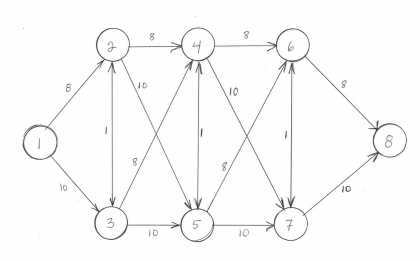
\includegraphics[width=12cm]{q3}
\end{figure}

Montrez le contenu du tableau \(D\), de l’ensemble \(S\) ainsi que la valeur de la variable \(v\) après chacune des itérations de l’algorithme. Décrivez toutes les étapes de l’algorithme Dijkstra. Utilisez le noeud 1 comme source.

\newpage

\section*{Question 4}
Résoudre les récurrences suivantes. \\

\textbf{a) } \(T(n)=2T\big(\frac{n}{2}\big)+1\) \\

\textbf{b) } \(T(n)=T\big(\frac{9n}{10}\big)+n\) \\

\textbf{c) } \(T(n)=16T\big(\frac{n}{4}\big)+n^2\) \\

\textbf{d) } \(T(n)=7T\big(\frac{n}{3}\big)+n^2\) \\

\textbf{e) } \(T(n)=7T\big(\frac{n}{2}\big)+n^2\) \\

\textbf{f) } \(T(n)=2T\big(\frac{n}{4}\big)+\sqrt{n}\) \\

\textbf{g) } \(T(n)=3T\big(\frac{n}{2}\big)+5n\) \\

\textbf{h) } \(T(n)=T\big(\frac{n}{2}+5\big)+1\) \\

\newpage

\section*{Question 5}
Considérez la matrice suivante
\begin{align*}
	F =
	\begin{pmatrix}
		0 & 1 \\
		1 & 1
	\end{pmatrix}
\end{align*}

Soit \(i\) et \(j\), deux entiers. Quel est le produit du vecteur (\(i\), \(j\)) et de la matrice \(F\)? Qu’arrive-t-il si i et j sont deux nombres consécutifs de la suite de Fibonacci? Utilisez cette idée pour concevoir un algorithme diviser-pour-régner capable de calculer le nième nombre de Fibonacci en temps \(\Theta (log \: n)\) en considérant (faussement) que les multiplications
prennent un temps constant. Expliquez le lien entre votre algorithme et l’algorithme fib3 du devoir 1. \newline

Il est possible de constater que le résultat de la multiplication suivante :
\begin{align*}
	\begin{pmatrix}
		f_{n-1} & f_{n-2}
	\end{pmatrix}
	\cdot
	\begin{pmatrix}
		0 & 1 \\
		1 & 1
	\end{pmatrix}
	=
	\begin{pmatrix}
		f_{n-1} & f_{n-1} + f_{n-2}
	\end{pmatrix}
\end{align*}

Il est possible de se rapeller l'identité de la séquence de Fibbonaci :
\[ f_{n} = f_{n-1} + f_{n-2} \]

Il est donc possible de remplacer une identité dans la première équation :
\begin{align*}
	\begin{pmatrix}
		f_{n-1} & f_{n-2}
	\end{pmatrix}
	\cdot
	\begin{pmatrix}
		0 & 1 \\
		1 & 1
	\end{pmatrix}
	=
	\begin{pmatrix}
		f_{n-1} & f_{n}
	\end{pmatrix}
\end{align*}

On remarque qu'on peut chaîner la multiplication de la matrice. On observe que l'indice de la séquence de Fibonacci augmente à chaque itération. On peut observer cela grâce aux équations suivantes.
\begin{align*}
	\begin{pmatrix}
		f_{0} & f_{1}
	\end{pmatrix}
	\cdot
	\begin{pmatrix}
		0 & 1 \\
		1 & 1
	\end{pmatrix}
	=
	\begin{pmatrix}
		f_{0} & f_{0} + f_{1}
	\end{pmatrix}
\end{align*}

\begin{align*}
	\begin{pmatrix}
		f_{1} & f_{2}
	\end{pmatrix}
	\cdot
	\begin{pmatrix}
		0 & 1 \\
		1 & 1
	\end{pmatrix}
	=
	\begin{pmatrix}
		f_{1} & f_{1} + f_{2}
	\end{pmatrix}
\end{align*}

En chaînant les multiplications par la matrice, on constate la relation suivante.
\begin{align*}
	\begin{pmatrix}
		f_{0} & f_{1}
	\end{pmatrix}
	\cdot
	\begin{pmatrix}
		0 & 1 \\
		1 & 1
	\end{pmatrix}
	^n
	=
	\begin{pmatrix}
		f_{n} & f_{n+1}
	\end{pmatrix}
\end{align*}

En remplacant \( f_{0} \) et \( f_{1} \) par leurs valeurs respectives.
\begin{align*}
	\begin{pmatrix}
		0 & 1
	\end{pmatrix}
	\cdot
	\begin{pmatrix}
		0 & 1 \\
		1 & 1
	\end{pmatrix}
	^n
	=
	\begin{pmatrix}
		f_{n} & f_{n+1}
	\end{pmatrix}
\end{align*}

\newpage

\section*{Question 6}
Soit \(X[1 \dots n]\) et \(Y [1 \dots n]\) deux tableaux, chacun contenant \(n\) nombres déjà triés. Donnez un algorithme diviser-pour-régner pour trouver le médian des \(2n\) éléments présents dans les tableaux \(X\) et \(Y\). Le temps d’exécution de votre algorithme doit être dans \(\Theta (log \: n)\) en pire cas.

\begin{flushleft}
L'algorithme suivant trouve la médiane de deux tableaux de même taille (taille `n`) de nombres triés. Il est à noter que la fonction `Mediane` utilisée aux lignes 7 et 8 est une fonction qui s'exécute en temps constant qui retourne la médiane d'un tableau.
\end{flushleft}


\begin{algorithm}[H]
      \KwData{\( X[1 \cdot\cdot\cdot  n], Y[1 \cdot\cdot\cdot  n], entier \: n \)}
      \KwResult{réel med}
      	\If{ \(n = 1\)}{
      		\Return \(  \big( \frac{X[1] + Y[1]}{2} \big) \) \
      	}

      	\If{ \(n = 2\)}{
      		\Return \(  \big( \frac{ max(X[1], Y[1]) + min(X[2], Y[2])   }{2} \big) \) \
      	}

      	\(medX \gets Mediane(X[1 \cdot\cdot\cdot  n]) \) \;
      	\(medY \gets Mediane(Y[1 \cdot\cdot\cdot  n]) \) \;

      	\If{\(medX = medY\)}{
      		\Return medX
      	}

      	\eIf{\(medX < medY\)}
      	{
      		\eIf{\( n\bmod  2 = 0\)}
      		{
      			\Return TrouverMédiane(X[\( \frac{n}{2} +1\) ...  n], Y[1 ...  \( \frac{n}{2} -1\)], \( \frac{n}{2} +1\))
      		}
      		{
      			\Return TrouverMédiane(X[\( \frac{n}{2}\) ...  n], Y[1 ...  \( \frac{n}{2}\)], \( \frac{n}{2}\))
      		}
      	}
      	{
      		      		\eIf{\( n\bmod  2 = 0\)}
      		{
      			\Return TrouverMédiane(X[1 ...  \( \frac{n}{2} -1\)], Y[\( \frac{n}{2} +1\) ...  n], \( \frac{n}{2} +1\))
      		}
      		{
      			\Return TrouverMédiane(X[\( \frac{n}{2}\) ...  n], Y[1 ...  \( \frac{n}{2}\)], \( \frac{n}{2}\))
      		}
      	}


      \caption{TrouverMédiane}
\end{algorithm}

\end{document}
